\section{Experimental evaluation}\label{sec:evaluation}
The evaluation examines three questions: whether switching bounds certify
updates that authenticated moments leave unresolved; whether those decisions
reduce total measured audit cost; and how decision coverage and assignment
quality vary across feature representations and learning workloads.
Numerical studies assess the certificate on additional fitted models.
Completed real-proof controls measure the cost of enforcing its relations.
These two forms of evidence are reported separately.

\subsection{Experimental protocol}
\subsubsection{Datasets and candidate updates}
The image experiments use MNIST and Fashion-MNIST
\cite{lecun1998,fashion2017}. Each fitted configuration separates training
rows from the committed audit catalog. Training-only Lloyd snapshots supply
the deployed centers and candidate banks. The frozen-profile confirmation
uses four new seeds per dataset, $k=5$, and deployed reference ages of one
and eight Lloyd steps. Its 1,024-record catalogs are held out from basis
fitting. Appendix~\ref{sec:protocol-spec} specifies source sampling,
quantization, clipping and the retained candidate grids.

The release-batch experiments add UCI smartphone activity features
(HAR, $D=561,k=6$) and 20 Newsgroups encoded with a frozen MiniLM transformer
($D=384,k=5$)~\cite{ucihar2012,news20data,minilmcard2026}. Official
training/test partitions are respected; the HAR source partitions separate
subjects. Each corpus has two row-disjoint fitted configurations, each
containing 500 past training records, 500 incoming training records and
1,024 held-out audit records. Past records alone determine scaling,
reference centers and bases. Each incoming 250-record minibatch supplies
assigned-group means; interpolation rates $0.25$, $0.5$ and $1.0$ yield six
candidate banks per configuration. All candidates are retained. Neural
features are owner-supplied committed inputs, with an archived encoder
revision and preprocessing hashes; encoder inference is outside the proof.

Prediction rank 63, certificate rank 79, basis precision 14 bits and an
exact-row cap of 16 are held fixed across the primary comparisons. These
values were selected during development. Later fits test that frozen
profile, while rank and cap sensitivity are reported separately. Catalog
prefixes, candidate rates and representations share data and are not
independent learning trials. Exact duplicate banks are cached before
outcomes are evaluated.

\subsubsection{Compared methods}
\paragraph{Centroid-informed and PCA certificates}
Both representations instantiate the same authenticated group relation,
rounded-basis switching bounds, refinement policy and paid fallback. They
receive the same training split, prediction and certificate ranks, precision,
catalog and candidates. The comparison isolates the basis construction;
PCA does not receive a weaker verification requirement.

\paragraph{Reusable exact Full}
Full authenticates original rows and evaluates exact quantized
nearest-center costs for centers disclosed after preprocessing. A common
circuit and setup are reused across candidate banks. The matched eight-worker
implementation batches eight rows per proof and uses cached keys and
buffered binary input/output. It is the exact reference for assignment
agreement and update-cost change.

\paragraph{Authenticated moments-only}
This baseline proves the projection-free group-target upper bound using
authenticated old groups, counts and sums. An unresolved request triggers
new Full proofs. It tests whether switching information adds enough decision
power to justify compact preprocessing and queries. It does not define an
approximate assignment predictor.

\paragraph{Exact affine controls}
Online affine constructs and authenticates scores for each currently
disclosed bank, charging each rebuild without access to later candidates.
Advance-bank affine instead knows the union of all evaluated centers before
preprocessing. It provides exact assignments and costs for that bank, but
has a different information contract. Its measurements are retained in
Appendix~\ref{sec:known-family-results} and are not used as timings for an
unseen-center service.

\paragraph{Alternative proof backend}
PLONK implements the exact Full relation on a bounded neural-text catalog.
The exported control uses test-only KZG parameters and is a backend execution
check. General zkML systems, GKR protocols, folding and proof aggregation
are related approaches rather than implemented matched baselines here
\cite{chen2024zkml,thaler2013time,kothapalli2022nova,gailly2022snarkpack}.

\subsubsection{Metrics and execution accounting}
For request $q$, let $y_{iq}$ be the exact quantized nearest-center label,
with lowest-index tie breaking, and $\widehat y_{iq}$ the approximate label.
Assignment agreement is
\begin{equation}\label{eq:evaluation-agreement}
 \operatorname{Agr}(q)=\frac{100}{N}\sum_{i=1}^{N}
       \mathbf1[\widehat y_{iq}=y_{iq}].
\end{equation}
Label-certificate coverage is the percentage of rows whose approximate
label is individually guaranteed. Update coverage is the number of
conclusive cost-change certificates before full-catalog fallback divided
by the number of requests. Regression coverage restricts that count to
requests with true $\Delta>0$. Mean agreement and label coverage average
request-level percentages; worst agreement is the lowest request value.
Neither agreement nor label-certificate coverage measures ground-truth
classification accuracy. Full and affine compute exact assignments by
construction, whereas moments-only has no corresponding prediction metric.

A valid interval can be inconclusive. This differs from a false conclusive
decision, which would contradict the sign of the independently computed
exact change. A working 99\% agreement target summarizes predictor quality;
it is not a threshold in the aggregate soundness argument. Numerical label
certificates are reported as quality diagnostics, rather than additional
public per-label proof outputs.

Proof controls run on an AMD Ryzen 7 5800H Windows laptop with eight physical
cores, 16 logical processors and approximately 13.9\,GiB usable RAM. Matched
controls use eight Go workers, a 1,200\,MiB soft memory target and a
3.5\,GiB process-RSS guard. Compact switching batches contain 16 records;
Full batches contain eight, under a 1.6-million-constraint guard. The
appendix records the scheduling and memory-policy amendments. Earlier
two-worker controls are identified separately; ratios are formed only
within matched workloads and execution settings.

Active time charges cold preprocessing, key work, native parameter
construction, proof generation, fresh public replay, recorded failed
attempts and newly generated exact fallback. Frozen representations and
encoder outputs are supplied to the primary controls as inputs; model
fitting is excluded consistently from their ratios. An already proved old
cost may be cached, but an unresolved request is not credited with an
unproved native answer. Speedup denotes matched Full time divided by method
time. Sleep-interrupted measurements remain in the records and are excluded
from clean timing conclusions.

\subsection{Certificate resolution and assignment quality}
\subsubsection{Contribution of switching information}
The retained MNIST development ablation contains 19 distinct updates with
15--56 strictly switching rows per update. Both the assigned-change test
and the stronger authenticated group-target moments upper bound resolve
2/19; the switching certificate resolves 19/19. This demonstrates the
additional decision power of switching information on that workload.
It is a development ablation rather than an independent confirmation set.

Natural worsening updates also require switching-aware reasoning. A mature
128-record MNIST control contains four regressions with 2, 7, 12 and 13
switching rows. The compact interval resolves three; two exact-row
corrections resolve the fourth. In the 1,024-record Fashion proof control,
all three worsening updates switch assignments (3, 9 and 10 rows) and are
certified by the centroid representation without corrections.

\subsubsection{Frozen-profile image confirmation}
Table~\ref{tab:review-quality} reports numerical results on the held-out
1,024-record catalogs. Centroid resolves all 60 image requests, including
all five observed regressions, without exact-row corrections. PCA reaches
the same decision coverage, using 14 corrected rows on Fashion. No
regression occurs in this MNIST confirmation set; its perfect update
coverage therefore does not independently measure regression detection.

Centroid's mean agreement is 99.948\% on Fashion and 99.942\% on MNIST,
compared with 99.916\% and 99.887\% for PCA. Its mean label-certificate
coverage is 98.982\% and 96.613\%, compared with 98.525\% and 95.990\%.
Both representations remain above 99\% agreement on every image request
in this confirmation. These are small representation differences within
a shared mechanism, rather than evidence of a universal centroid advantage.
\begin{table*}[tbp]
\centering
\caption{Native quality on 1,024-record catalogs. Image rows pool four new seeds and deployed ages 1/8; HAR and neural text pool two row-disjoint fitted configurations with six new-training-minibatch proposals each. HAR uses six centers and neural text five. Coverage is before full-catalog fallback. Agreement, individual-label certificates and update decisions concern different outputs. Below 99 counts requests missing the working agreement target; 0/0 means no regression occurred.}
\label{tab:review-quality}
\begin{adjustbox}{max width=.98\textwidth,center=\textwidth}
\begin{tabular}{llrrrrrrr}
\toprule
Data & Basis & Updates & Regressions & Mean agr. & Worst & Label cert. & Exact rows & Below 99\\
\midrule
Fashion & Centroid & 28/28 & 5/5 & 99.948 & 99.805 & 98.982 & 0 & 0\\
Fashion & PCA & 28/28 & 5/5 & 99.916 & 99.707 & 98.525 & 14 & 0\\
MNIST & Centroid & 32/32 & 0/0 & 99.942 & 99.707 & 96.613 & 0 & 0\\
MNIST & PCA & 32/32 & 0/0 & 99.887 & 99.609 & 95.990 & 0 & 0\\
HAR & Centroid & 11/12 & 3/4 & 99.691 & 99.023 & 92.871 & 24 & 0\\
HAR & PCA & 11/12 & 3/4 & 99.642 & 98.926 & 91.829 & 23 & 1\\
Neural text & Centroid & 8/12 & 0/4 & 96.370 & 92.188 & 28.743 & 64 & 12\\
Neural text & PCA & 8/12 & 0/4 & 95.793 & 91.992 & 22.176 & 64 & 12\\
\bottomrule
\end{tabular}
\end{adjustbox}
\end{table*}


\subsubsection{Sensor and neural-text release batches}
On HAR, both representations certify 11/12 requests and 3/4 regressions
before complete-catalog fallback. Centroid averages 99.691\% agreement,
with a worst request of 99.023\% and 92.871\% mean label coverage. PCA
averages 99.642\% agreement, with a worst value of 98.926\% and 91.829\%
label coverage. Thus centroid meets the working agreement target on every
HAR request, while PCA misses it on one. The remaining update requires
exact fallback to resolve its sign.

Neural text exposes a less favorable geometry. Both bases certify 8/12
requests, but all four naturally worsening full-step updates remain
inconclusive. Centroid's mean and worst agreement are 96.370\% and
92.188\%, compared with 95.793\% and 91.992\% for PCA. Mean label coverage
is only 28.743\% and 22.176\%, respectively. All twelve centroid requests
miss the working 99\% agreement target. The valid intervals therefore
retain correctness while providing insufficient resolution for the
regressions in this workload. The numerical coverage figures do not imply
a measured end-to-end proof speedup for HAR or text.
% Neural activity diagnostic is unfinished; no result is reported.


\subsection{Measured runtime and exact baselines}
\subsubsection{Complete certificate--Full comparisons}
Table~\ref{tab:optimized-proofs} gives the completed primary method--Full
pairs. On Fashion with 1,024 records, centroid certifies the three
regressions in 42.534 minutes, PCA in 44.156 minutes and exact Full in
101.575 minutes. Their matched Full/method ratios are 2.388 and 2.300.
Centroid uses 57.2\% less active time than Full in this execution. PCA
requires three exact-row corrections; centroid requires none.

Moments-only resolves no request before fallback and costs 134.413 minutes,
including the new exact proofs. Thus its lower-cost query does not produce
a lower total service cost on this workload. The decisive factor is the
frequency with which a certificate avoids full-catalog evaluation.

The two 128-record MNIST fits have three matched repetitions each.
Centroid's median speedups are 1.986 and 2.004; PCA's are 1.993 and 1.996.
These differences do not support a consistent runtime ordering between the
two bases. Moments-only reaches median ratios of 0.764 and 1.000, reflecting
its unresolved requests and fallback cost. The Fashion headline has one
execution, so no timing-variation interval is inferred for its 2.388 ratio.
\begin{table*}[tbp]
\centering
\caption{Completed method--Full pairs, eight workers, frozen fitted models supplied as inputs; fitting is excluded consistently. Case identifies dataset and $k$/seed/reference Lloyd step. Reps counts completed pairs for that method, not completion of every baseline. Ratios include preprocessing, keys, recorded attempts, generation, public replay and newly paid fallback (FB). Repeated decisions share the same fit and proposals.}
\label{tab:optimized-proofs}
\begin{adjustbox}{max width=.98\textwidth,center=\textwidth}
\begin{tabular}{lrlrrrrrrr}
\toprule
Case & $N$ & Method & Reps & Full min. & Method min. & Range & Full/method & Decisions & FB\\
\midrule
Fashion 5/173/8 & 1024 & Centroid & 1 & 101.575 & 42.534 & 42.534--42.534 & 2.388 & 3/3 & 0\\
Fashion 5/173/8 & 1024 & Moments-only & 1 & 101.575 & 134.413 & 134.413--134.413 & 0.756 & 0/3 & 3\\
Fashion 5/173/8 & 1024 & PCA & 1 & 101.575 & 44.156 & 44.156--44.156 & 2.300 & 3/3 & 0\\
MNIST 3/101/8 & 128 & Centroid & 3 & 20.475 & 10.176 & 8.705--11.095 & 1.986 & 12/12 & 0\\
MNIST 3/101/8 & 128 & Moments-only & 3 & 20.475 & 24.107 & 22.632--28.849 & 0.764 & 0/12 & 12\\
MNIST 3/101/8 & 128 & PCA & 3 & 20.475 & 10.242 & 8.673--11.145 & 1.993 & 12/12 & 0\\
MNIST 5/173/8 & 128 & Centroid & 3 & 17.501 & 8.734 & 8.734--8.734 & 2.004 & 12/12 & 0\\
MNIST 5/173/8 & 128 & Moments-only & 3 & 17.501 & 17.495 & 17.438--17.555 & 1.000 & 6/12 & 6\\
MNIST 5/173/8 & 128 & PCA & 3 & 17.501 & 8.767 & 8.750--8.767 & 1.996 & 12/12 & 0\\
\bottomrule
\end{tabular}
\end{adjustbox}
\end{table*}

% No new learning-workload proof pair has completed.


\subsubsection{Affine and backend controls}
The request-local online affine controls cost 23.104 and 19.211 minutes,
compared with matched Full times of 21.868 and 17.468 minutes
(Table~\ref{tab:optimized-exact}). Authenticating a newly disclosed bank
therefore costs approximately 6--10\% more than Full in these two controls.
These are separate executions; their absolute times are not combined with
other repetitions to create an additional speedup ratio.
\begin{table*}[tbp]
\centering
\caption{Completed exact controls, one execution per fit and runtime setting. Online affine rebuilds for each currently disclosed bank with no future-center bank. Full/control compares matched active costs including fresh public replay.}
\label{tab:optimized-exact}
\begin{adjustbox}{max width=.98\textwidth,center=\textwidth}
\begin{tabular}{llrrr}
\toprule
Case & Exact control & Full min. & Control min. & Full/control\\
\midrule
MNIST 3/101/8 & Online affine & 21.868 & 23.104 & 0.947\\
MNIST 5/173/8 & Online affine & 17.468 & 19.211 & 0.909\\
\bottomrule
\end{tabular}
\end{adjustbox}
\end{table*}


Advance knowledge can change the preferred exact method. The supplementary
advance-bank control completes the 128-record mature MNIST workload in
4.710 minutes and its 1,024-record MNIST scale workload in 44.704 minutes
(Table~\ref{tab:known-family}). Those exact results show why an audit service
should exploit a genuinely known future bank. They do not provide the cost
of answering an arbitrary center request that arrives after preprocessing.

The exported PLONK control covers 64 genuine neural-text records and seven
center banks, producing 448 exact proofs. Batch size one is selected for
laptop feasibility, and the catalog prefix is chosen using pilot runtime
before inspecting certificate outcomes. The current exported timing is
sleep-interrupted and supports no clean backend speed ranking
(Table~\ref{tab:review-backend}). Test-only cached KZG parameter creation is
recorded separately; the control charges parameter loading, circuit setup,
proving and fresh public replay. Its unsafe benchmark parameters do not
establish production soundness. A compiled circuit or a numerical result is
not substituted for a completed backend comparison.
\begin{table*}[tbp]
\centering
\caption{Completed exact Full controls on the same 64-record neural-text catalog and seven banks. Every exact batch and complete row coverage are independently checked; public proofs are replayed. Active time includes replay. Test-only cached KZG parameters are unsafe for deployment; creation is separate, while runs charge loading, circuit setup and proving. Interrupted timing is excluded from comparisons. Groth16 batch 1 separates backend from batching; larger feasible PLONK batches are retained when completed. Repetitions share one fitted model.}
\label{tab:review-backend}
\begin{adjustbox}{max width=.98\textwidth,center=\textwidth}
\begin{tabular}{lrlrrrrr}
\toprule
Backend & Batch & Execution & Proofs & Active min. & Replay s & Proof MiB & Setup s\\
\midrule
PLONK & 1 & repetition\_01 & 448 & \emph{interrupted} & 6.309 & 0.250 & 1.443\\
\bottomrule
\end{tabular}
\end{adjustbox}
\end{table*}


\subsection{Proof traffic, verification and timing variation}
Table~\ref{tab:review-resources} reports measured cryptographic proof bytes,
verification-key size, fresh public replay and peak prover RSS. On Fashion,
centroid produces 1,219 proofs totaling 0.228\,MiB, compared with 512 proofs
and 0.096\,MiB for Full. Public replay takes 20.927 seconds for centroid
and 4.615 seconds for Full. PCA produces 1,222 proofs and takes 44.142
seconds for replay. Compact audit computation consequently saves total
active time while increasing the number of proofs and verifier work.
Proof bytes exclude public witnesses, metadata and transfer overhead.

Peak prover RSS is 1.412\,GiB for centroid, 1.420\,GiB for PCA and
2.057\,GiB for Full in the same Fashion comparison. These are maxima over
the measured phases under the stated guards, rather than memory-scaling
curves or aggregate memory consumption across arbitrary deployments.
\begin{table*}[tbp]
\centering
\caption{Cold public artifacts and resource costs for completed comparisons (first execution per fit). Proof MiB counts cryptographic proof bytes; VK KiB counts exported verification keys. Replay is a fresh public-only verifier pass. RSS is the largest measured prover-process resident set across preprocessing, setup, queries, correction and paid fallback. Public witnesses, model metadata and transfer time are separate from proof bytes.}
\label{tab:review-resources}
\begin{adjustbox}{max width=.98\textwidth,center=\textwidth}
\begin{tabular}{lrrrrr}
\toprule
Case/method & Proofs & Proof MiB & VK KiB & Replay s & Peak GiB\\
\midrule
MNIST128/Full & 80 & 0.015 & 74.4 & 0.584 & 1.970\\
MNIST128/Centroid & 166 & 0.031 & 166.3 & 10.833 & 1.174\\
MNIST128/PCA & 167 & 0.031 & 166.3 & 11.527 & 1.174\\
Fashion 1024/Full & 512 & 0.096 & 123.4 & 4.615 & 2.057\\
Fashion 1024/Centroid & 1219 & 0.228 & 138.9 & 20.927 & 1.412\\
Fashion 1024/PCA & 1222 & 0.228 & 275.4 & 44.142 & 1.420\\
\bottomrule
\end{tabular}
\end{adjustbox}
\end{table*}


Table~\ref{tab:review-uncertainty} gives variation across the three serial
executions per MNIST fit. The conditional log-ratio intervals use a
Student $t$ calculation with two degrees of freedom. They describe host
and execution variation for fixed fitted models; they do not estimate
variation across independent datasets or learning problems. The distinction
is material because many requests share the same training fit, reference
bank and preprocessing.
\begin{table*}[tbp]
\centering
\caption{Timing variability conditional on one fit and host. Ratios include all measured active components. SD is across three serial executions; the log-ratio Student t interval is descriptive under a normal-log-ratio assumption with only two degrees of freedom. It is not an interval across datasets or independent learning trials.}
\label{tab:review-uncertainty}
\begin{adjustbox}{max width=.98\textwidth,center=\textwidth}
\begin{tabular}{llrrrr}
\toprule
Case & Method & Reps & Median ratio & SD & Conditional 95\% interval\\
\midrule
MNIST3/101/8 & Centroid & 3 & 1.986 & 0.021 & 1.939--2.042\\
MNIST3/101/8 & PCA & 3 & 1.993 & 0.020 & 1.936--2.035\\
MNIST3/101/8 & Moments-only & 3 & 0.764 & 0.051 & 0.674--0.924\\
MNIST5/173/8 & Centroid & 3 & 2.004 & 0.005 & 1.993--2.017\\
MNIST5/173/8 & PCA & 3 & 1.996 & 0.003 & 1.990--2.007\\
MNIST5/173/8 & Moments-only & 3 & 1.000 & 0.006 & 0.986--1.015\\
\bottomrule
\end{tabular}
\end{adjustbox}
\end{table*}


\subsection{Sensitivity, scale and reuse economics}
\subsubsection{Certificate rank and exact-row budget}
Table~\ref{tab:review-rank-cap} varies certificate rank and correction cap
on the first declared 128-record fit per added corpus, keeping prediction
rank and precision fixed. HAR resolves 5/6 requests without corrections
at ranks 39, 63 and 79. Four corrections increase coverage to 6/6 at rank
79; larger budgets add no decision. Neural text remains at 4/6 even with
32 corrections. These cases neither establish rank 79 as necessary nor
identify an optimal correction budget. The selected profile is a frozen
resource choice, and geometry determines whether its additional work
improves resolution.
\begin{table*}[tbp]
\centering
\caption{Controlled native rank/cap ablation on the first declared fit per added corpus, N128, all six minibatch proposals. Prediction rank 63 and precision 14 stay fixed; only certificate rank and correction budget change. Each cell gives resolved updates. Ranks 39/63/79 use prefixes of the same frozen training basis. These are numerical resolution counts, not measured proof-speed ratios.}
\label{tab:review-rank-cap}
\begin{adjustbox}{max width=.98\textwidth,center=\textwidth}
\begin{tabular}{llrrrrrr}
\toprule
Data & Basis & 39/0 & 63/0 & 79/0 & 79/4 & 79/16 & 79/32\\
\midrule
HAR & Centroid & 5/6 & 5/6 & 5/6 & 6/6 & 6/6 & 6/6\\
HAR & PCA & 5/6 & 5/6 & 5/6 & 6/6 & 6/6 & 6/6\\
Neural text & Centroid & 4/6 & 4/6 & 4/6 & 4/6 & 4/6 & 4/6\\
Neural text & PCA & 4/6 & 4/6 & 4/6 & 4/6 & 4/6 & 4/6\\
\bottomrule
\end{tabular}
\end{adjustbox}
\end{table*}


\subsubsection{Numerical scale and reference reuse}
The supplementary native series evaluates genuine held-out prefixes through
16,384 records, with a primary age-one series and retained age-eight
diagnostics (Table~\ref{tab:optimized-scale}). Both bases resolve the
reported requests in that series. These results measure numerical decision
quality; the evaluated catalog size is not evidence of completed
16,384-record proving performance. The measured image proof controls use
small center counts, and do not establish practical scaling to many centers.

For $m$ requests against one deployed reference, write $P$ for cold
preparation and key work, $Q_j$ for request work including corrections and
replay, and $F_j$ for newly generated exact fallback. Then
\begin{equation}\label{eq:service-cost}
 C_{\mathrm{active}}(m)=P+\sum_{j=1}^{m}Q_j
                     +\sum_{j\in\mathcal U_m}F_j,
\end{equation}
where $\mathcal U_m$ contains requests left unresolved by the bounded
certificate path. Both unsuccessful certificate attempts and paid fallback
remain in this total. Figure~\ref{fig:cost-frontier} uses measured components
from the earlier two-worker, 19-request MNIST workload to show cumulative
allocation and modeled reference replacement. Intermediate prefixes and
reset curves are allocations or models, rather than new deployment runs.
\begin{figure*}[tbp]
\centering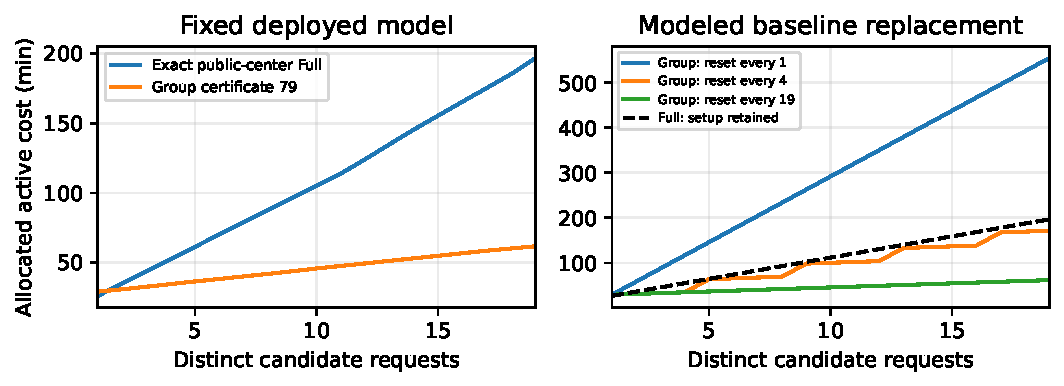
\includegraphics[width=.94\textwidth]{paper_results/referee_final_20261025/generated/cost_frontier.pdf}
\caption{Cost accounting from completed two-worker MNIST components. Left: fixed-baseline cumulative allocation, with measured replay, key-loading and other residual overhead charged upfront. The 19-request endpoints equal recorded active totals; intermediate prefixes are allocations, not fresh runs. Right: modeled repeated cold group preparation versus reusable Full setup, using measured mean query components. Reset curves are not measured rebase deployments and do not include newly fitted bases.}
\label{fig:cost-frontier}
\end{figure*}


A release batch shares $P$ while comparing candidates. Installing one
candidate as the new deployed reference requires fresh group preprocessing,
whereas Full's public-center setup can remain reusable. The method is
therefore most attractive when several useful decisions share a reference
and the compact intervals rarely require complete fallback. Frequent
reference replacement or difficult switching geometry can remove that
advantage even when every accepted certificate remains correct.
